\documentclass[tikz,border=6pt]{standalone}
\usepackage{pgfplots}
\usepackage{amsmath}
\usetikzlibrary{
  arrows.meta,
  backgrounds,
  calc,
  fit,
  matrix,
  positioning,
  shapes.callouts,
  shapes.geometric,
  shapes.misc
}
\pgfplotsset{compat=1.18}

\definecolor{archInk}{HTML}{1F2933}
\definecolor{archBlue}{HTML}{0B4F6C}
\definecolor{archTeal}{HTML}{1B998B}
\definecolor{archGold}{HTML}{D98E04}
\definecolor{archRose}{HTML}{C44536}
\definecolor{archSage}{HTML}{7A9E7E}
\definecolor{archMist}{HTML}{E9F1F7}
\definecolor{archSand}{HTML}{F4F1DE}
\definecolor{archSlate}{HTML}{5C677D}
\definecolor{archStone}{HTML}{C8D0D9}

\tikzset{
  every node/.style={font=\sffamily\small, text=archInk},
  axis label/.style={font=\sffamily\footnotesize, text=archInk},
  panel/.style={
    rounded corners=6pt,
    draw=archSlate,
    line width=0.9pt,
    fill=white
  },
  stage/.style={
    panel,
    fill=archMist,
    minimum height=1.5cm,
    inner sep=7pt,
    align=left
  },
  note/.style={
    panel,
    fill=archSand,
    inner sep=7pt,
    align=left
  },
  verdict/.style={
    panel,
    fill=archTeal!12,
    inner sep=7pt,
    align=left
  },
  kill/.style={
    panel,
    fill=archRose!12,
    draw=archRose,
    inner sep=7pt,
    align=left
  },
  muted/.style={
    panel,
    fill=archStone!20,
    draw=archStone!80!archInk,
    inner sep=6pt,
    align=left
  },
  link/.style={
    -{Latex[length=3mm,width=1.7mm]},
    line width=1.0pt,
    draw=archBlue
  },
  dashedlink/.style={
    -{Latex[length=3mm,width=1.7mm]},
    line width=1.0pt,
    draw=archRose,
    dashed
  }
}

\pgfplotsset{
  every axis/.append style={
    line width=0.9pt,
    tick style={draw=archSlate},
    axis line style={draw=archSlate},
    label style={font=\sffamily\small, text=archInk},
    ticklabel style={font=\sffamily\footnotesize, text=archInk},
    legend style={
      draw=none,
      fill=white,
      font=\sffamily\footnotesize,
      text=archInk
    },
    title style={font=\sffamily\small\bfseries, text=archInk},
    grid style={draw=archStone},
    major grid style={draw=archStone},
    minor grid style={draw=archStone!70}
  }
}

\begin{document}
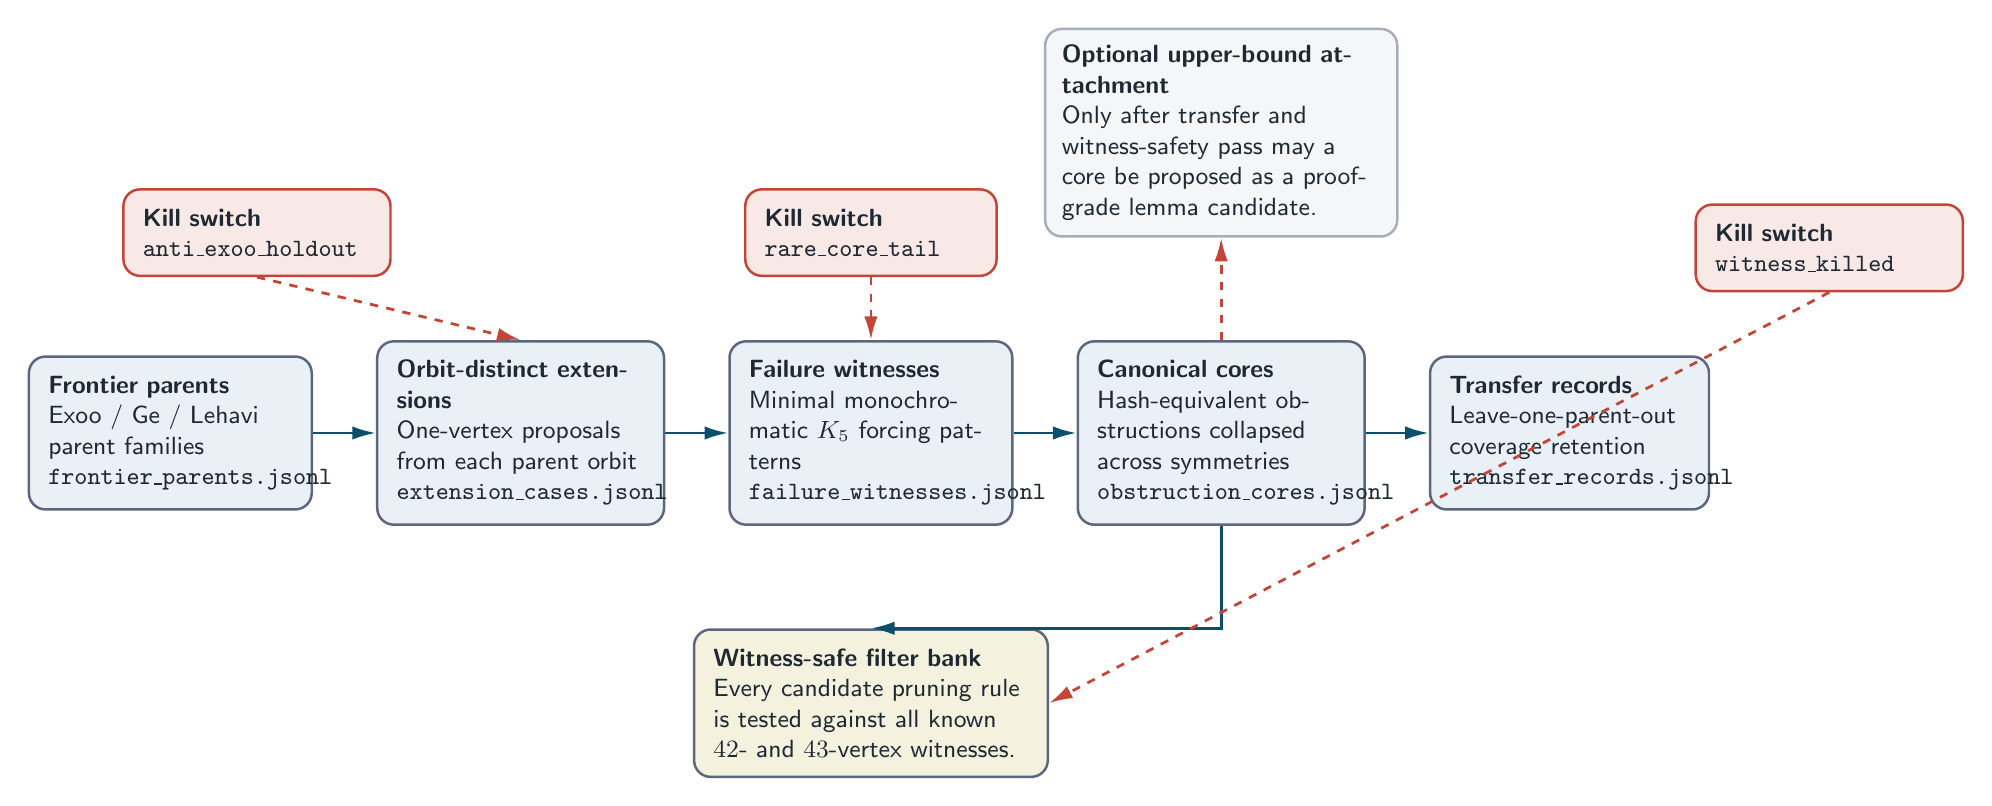
\begin{tikzpicture}[node distance=9mm and 8mm]
  \node[stage, text width=3.1cm] (parents) {
    \textbf{Frontier parents}\\
    Exoo / Ge / Lehavi parent families\\
    \texttt{frontier\_parents.jsonl}
  };
  \node[stage, text width=3.15cm, right=of parents] (extensions) {
    \textbf{Orbit-distinct extensions}\\
    One-vertex proposals from each parent orbit\\
    \texttt{extension\_cases.jsonl}
  };
  \node[stage, text width=3.1cm, right=of extensions] (witnesses) {
    \textbf{Failure witnesses}\\
    Minimal monochromatic $K_5$ forcing patterns\\
    \texttt{failure\_witnesses.jsonl}
  };
  \node[stage, text width=3.15cm, right=of witnesses] (cores) {
    \textbf{Canonical cores}\\
    Hash-equivalent obstructions collapsed across symmetries\\
    \texttt{obstruction\_cores.jsonl}
  };
  \node[stage, text width=3.05cm, right=of cores] (transfer) {
    \textbf{Transfer records}\\
    Leave-one-parent-out coverage retention\\
    \texttt{transfer\_records.jsonl}
  };

  \draw[link] (parents) -- (extensions);
  \draw[link] (extensions) -- (witnesses);
  \draw[link] (witnesses) -- (cores);
  \draw[link] (cores) -- (transfer);

  \node[note, text width=4cm, below=13mm of witnesses] (filterbank) {
    \textbf{Witness-safe filter bank}\\
    Every candidate pruning rule is tested against all known $42$- and $43$-vertex witnesses.
  };
  \draw[link] (cores.south) |- (filterbank.north);

  \node[muted, text width=4.05cm, above=13mm of cores] (lemma) {
    \textbf{Optional upper-bound attachment}\\
    Only after transfer and witness-safety pass may a core be proposed as a proof-grade lemma candidate.
  };
  \draw[dashedlink] (cores.north) -- (lemma.south);

  \node[kill, text width=2.9cm, above left=8mm and -2mm of extensions] (kill1) {
    \textbf{Kill switch}\\
    \texttt{anti\_exoo\_holdout}
  };
  \node[kill, text width=2.7cm, above=8mm of witnesses] (kill2) {
    \textbf{Kill switch}\\
    \texttt{rare\_core\_tail}
  };
  \node[kill, text width=2.9cm, above right=8mm and -2mm of transfer] (kill3) {
    \textbf{Kill switch}\\
    \texttt{witness\_killed}
  };

  \draw[dashedlink] (kill1.south) -- (extensions.north);
  \draw[dashedlink] (kill2.south) -- (witnesses.north);
  \draw[dashedlink] (kill3.south) -- (filterbank.east);
\end{tikzpicture}
\end{document}
